%!TEX root = ../Thesis.tex
% Chapter Template

\chapter{Design \& development} % Main chapter title

\label{DesignDevelopment} % Change X to a consecutive number; for referencing this chapter elsewhere, use \ref{ChapterX}

\lhead{Chapter \ref{DesignDevelopment}. \emph{Design \& Development}} % Change X to a consecutive number; this is for the header on each page - perhaps a shortened title

%----------------------------------------------------------------------------------------
% SECTION 1
%----------------------------------------------------------------------------------------
This chapter will briefly touch on the development of both the \CTC algorithm and genetic algorithm. The chapter will then go into some detail about the design of the algorithms so that the reader may better understand the code and how the algorithms work. This chapter will also be of benefit to those who wish to use the genetic optimisation algorithm or even modify it. The chapter will also explain some of the theory behind the \CTC algorithm functions and clearly specify the parameters of the \CTC algorithm as the clustering process is explained.

\section{Stages of development}
The addition of a genetic optimisation algorithm to the thesis goal necessitated some development. The \CTC algorithm authored by \cite{Moe2014} is implemented in Python and use a statically defined algorithm design. This necessitated some modification of the existing implementation to make it possible to dynamically specify algorithm designs. The code is reimplemented in Python 3 and amended to provide easy ways to execute the genetic algorithm.

% I had no familiarity with Python. The \emph{first stage} of development was thus to learn Python and familiarise myself with the implementation of the \CTC algorithm. The algorithm was implemented with largely hard coded parameters with about one separate python module (file) for each parameter configuration. To make testing different parameter sets easier a \emph{second stage} of development was performed. The parameter set were abstracted away so that the clustering function would accept any parameter set. This made it possible to perform initial incremental tests. These incremental tests then informed the design of the genetic algorithm, the \emph{third stage} of development. The genetic algorithm was initially developed to run on a single computer and was designed following the specifications in \cite{Goldberg1989,Negnevitsky2002,Haupt2004a}. Testing of the initial design for the genetic algorithm revealed that it was indeed capable of improving the F-Measure of the \CTC algorithm's results. There were a problem however as testing many chromosomes on a single machine took too much time. It was necessary to distribute the task.

% A \emph{fourth stage} of development was executed to alleviate the problem. A small server - client framework was written to facilitate distribution of computation tasks. The genetic algorithm was then rewritten to send chromosomes (essentially parameter sets) to clients that would then perform the actual clustering tasks. This made it very simple to run the clustering job on multiple CPU cores and multiple computers. Additionally a corpus processor was implemented to convert other corpus files to the snippet format used for the \CTC algorithm. A new subclass of the corpus processor needs to be implemented for each additional corpus to be converted.

% \subsection{Memory handling}
% One problem with Python 2 is the way it handles memory. The client processes would, at least in some environments, consistently eat up as much memory as they could and never free up memory used. This seemed to be a problem related to the way in which Python 2 allocates and deallocates memory for small variables such as integers. Essentially the Python 2 virtual machine would hold on to memory space allocated to small variables in case it could need such space later. This in essence saves CPU cycles as it does not have to ask for more space later. The problem seemed to be that it did not reuse that space later, but instead opted to ask for a new virtual memory space for small variables. Because of this the entire project had to be ported to Python 3.

Porting the \CTC algorithm from Python 2 to Python 3 proved to be an issue. The original \CTC implementation had produced consistent results. After porting the algorithm from Python 2 to Python 3, the algorithm started producing slightly varying results between test runs. It turns out that the problem was caused by the use of dictionaries (\texttt{dict} type). This use was affected by the transition from Python 2 to Python 3. In Python 2 the order in which items (key-value pairs) are inserted into a dictionary is stored implicitly\footnote{\url{http://docs.python.org/2.7/library/stdtypes.html\#dict}}. When you iterate through the items in the dictionary, they are extracted in the same order as they were inserted. This is not true for the Python 3 implementation of dictionaries. In Python 3 you are given a view\footnote{\url{http://docs.python.org/3.3/library/stdtypes.html\#dict}} when you ask for an iterator over the items in the dictionary, and this view does not necessarily give you the items in the same order as they were inserted. The solution was to implement the compact trie subtree dictionaries as \texttt{OrderedDict}\footnote{\url{http://docs.python.org/3.3/library/collections.html\#collections.OrderedDict}} objects to get the same order each time. This ensures that the resulting base clusters are the same on each run of the algorithm and thus secure the consistency of the clustering results.

\section{Overview of system}
This section will give an overview of the algorithms. It will cover the overall design of the algorithms and diverge briefly into some technical aspects. The code base of the project is too big to be covered in its entirety. The code is open source and can be found in full at \href{http://github.com/snorremd/distributed-clustering}{GitHub - http://github.com/snorremd/distributed-clustering}. The code is licensed under the MIT license which means that it can be used and modified freely.

\subsection{\CTC}
TThe \CTC algorithm is implemented as a class. The class initialiser (similar to a constructor) takes as parameters a \texttt{Corpus} object, that specifies which corpus is to be used, and a \texttt{ClusterSettings} object that informs the \CTC object which value to use for the beta constant for the F-Measure. This measure was discussed in Chapter~\ref{Theory}. The beta constant can be used to tune the kind of results the genetic algorithm optimise for by weighing either precision or recall higher than the other. In this thesis the harmonious F-Measure has been used for reasons of neutrality.

The initialiser continues by building an index of ground truth clusters, a tag-index, and indexes over different frequency measures (corpus frequency, raw frequency and document frequency) for the terms contained within the corpus. The raw frequency of a term is the number of times that term occurs in the corpus. The ground truth index and tag index are both created based on the snippet file specified in the \texttt{Corpus} object. These frequencies are later used for some of the similarity measures. The snippet file is marked up in XML and use the structure shown in Listing~\ref{lst:snippetfile}.
Essentially the snippet file encompasses an entire corpus. It is divided into snippet elements which correspond to one document. Each snippet is then divided into text type elements which comprise one of six forms of text from that document. Each text type element, for example ``ArticleText'', then holds snip elements that are of that text type. Ground truth clusters are then the documents that have equal tag-values. The tag index is an index of sources (documents) pointing to the tag value of that document. It is built by collecting the source and tag-values of each document.

\begin{lstlisting}[float=ht, language=xml, breaklines=true, label=lst:snippetfile, caption={Snippet file encoded in XML}]
<?xml version='1.0' encoding='ascii'?>
<snippetcollection source="klimaukenOBT.xml">
    <snippet id="2009-12-07-aa-01" source="http://www.adressa.no/nyheter/trondheim/article1419658.ece" tags="Innenriks-ulykker-trafikk-utforkj&#248;ring-trondheim">
        <ArticleIntroduction>
            <snip> bil havne bokstavelig tale hel kant Nedre Elvehavn mandag ettermiddag</snip>
        </ArticleIntroduction>
        <ArticleText>
            <snip> bil havne hel kant Nedre Elvehavn mandag ettermiddag</snip>
            <snip> bil tom</snip>
            <snip> If&#248;lge politi S&#248;r-Tr&#248;ndealg skulle bil tom komme sted</snip>
            <snip> menneske bil politi komme</snip>
            <snip> brannvesen sikre bil Falck rekvirere berging fortelle Curt Ivar R&#248;hmen operasjonsleder S&#248;r-Tr&#248;ndelag politidistrikt</snip>
            <snip> st&#229; fri</snip>
            ...
        </ArticleText>
        <ArticleByline>
            <snip> Tore Lagesen helle bil nesten ende vann Nedre Elvehavn</snip>
        </ArticleByline>
        <ArticleHeading>
            <snip> Biltur hel kant</snip>
        </ArticleHeading>
        <FrontPageIntroduction>
            <snip> En bileier Trondheim flaks side bil ta tur h&#229;nd mandag ettermiddag</snip>
            <snip> le mye</snip>
        </FrontPageIntroduction>
        <FrontPageHeading>
            <snip> telefon bil tur elv</snip>
        </FrontPageHeading>
    </snippet>
    <snippet>
      ...
    </snippet>
    ...
  </snippetcollection>
\end{lstlisting}

The \CTC algorithm is implemented as a method named \texttt{clustering} in the \texttt{CompactTrieClusterer} class. The application applies a \texttt{chromosome}, which essentially act as a parameter set (see Listing~\ref{lst:chromosome}), to the method and then executes each step of the \CTC algorithm according to the parameter values supplied. The method takes a number of parameters each of which will be explained in the coming sections. A list is provided below to give an overview of all the identified parameters.
\begin{description}
\item[Tree type]\hfill \\The tree type (suffix, mid-gram, etc) used to build the phrase tree.
\item[Top Base Clusters]\hfill \\The top base clusters limit that determines the amount of base clusters to include for base cluster merging.
\item[Min term occurrence]\hfill \\The minimal number of occurrences of a term in the corpus for it to not be considered a stop word.
\item[Max term ratio]\hfill \\The maximal allowed ratio of a term in the corpus for it not to be considered a stop word.
\item[Min limit base cluster score]\hfill \\The lower limit at which the base cluster label is scored the minimum score.
\item[Max limit base cluster score]\hfill \\The upper limit at which the base cluster label is scored the maximum score.
\item[Order descending]\hfill \\Whether to order the base clusters list in descending or ascending order.
\item[Drop singleton base clusters]\hfill \\Whether to drop singleton base clusters or not.
\item[Drop one word clusters]\hfill \\Whether to drop one word clusters or not.
\item[Text types]\hfill \\Which kinds of text to include in the snippet expansion phase.
\item[Text amount]\hfill \\The amount of article text to include in the snippet expansion phase.
\item[Similarity method]\hfill \\Which similarity method to use in the base clusters similarity function.
\end{description}.

\begin{lstlisting}[float=ht!, language=python, label=lst:chromosome, caption={An example chromosome}]
fitness = 0
id = 1
idCounter = 2
results = ## Ommitted
tree_type = (0,0,0)
top_base_clusters_amount = 992
min_term_occurence_in_collection = 23
max_term_ratio_in_collection = 0.72
min_limit_for_base_cluster_score = 3
max_limit_for_base_cluster_score = 7
should_drop_singleton_base_clusters= 0
should_drop_one_word_clusters = 1
text_amount = 0.73
text_types = {
  "FrontpageIntroduction": 1,
  "FrontpageHeading": 0,
  "ArticleHeading": 1,
  "ArticleByline": 1,
  "ArticleIntroduction": 0,
  "ArticleText": 1
}
similarity_measure = {
  similarity_method: 2,
  params: (0.5, 10, 1)
}
descending_order: 1
\end{lstlisting}

\subsubsection{Snippet filtering}
\label{subsubsec:snippetfiltering}
The first step in the \CTC algorithm is snippet filtering. The algorithm filters the snippet list according to which \emph{text types} should be included. Because the parameter is randomised there are cases where the chromosome specifies that no text types should be included. In such cases the algorithm returns an empty result. An empty result is a result were each performance measure is given a score of zero. The chromosome also specify a \emph{text amount} ratio that tells the algorithm how much of the article text to include. This ratio is in the range 0 \dots 1 with a .01 increment. In the event that article text should be included the number of sentences to include are then simply calculated by multiplying the number of article text sentences with the ratio.

\subsubsection{Snippet expansion}
\label{subsubsec:snippetexpansion}
The algorithm then moves on to the snippet expansion phase. It selects the expansion technique given by the \emph{tree type} parameter in the chromosome. Research shows that it is possible to achieve results with n-grams comparable to suffixes, but in less time, \parencite{Moe2013compact,Moe2014}. The expansion technique (tree type) may be one of the following: suffix, n-gram, mid-gram or range-gram expansion. Each expansion technique will be explained with an example. Given a snippet \(S\): ``mouse run trough house order find cheese is discovered cat chase away'', we can define the snippet as \(S = t_{1} \dots t_{12}\). \(S\) can be expanded using each of the four expansion techniques described below.

Each suffix phrase \(P\)  of \(S\) are defined as: \(P = t_{12-m+1} \dots t_{12}\) where \(0 \le m < 12\). This gives us the following suffixes for the snippet: \textit{1}) ``mouse run through house order find cheese is discovered cat chase away'', \textit{2}) ``run through house order find cheese is discovered cat chase away'', \textit{3}) ``through house order find cheese is discovered cat chase away'', \textit{4}) ``house order find cheese is discovered cat chase away'', ..., \textit{11}) ``chase away'', and \textit{12}) ``way''.


A n-gram phrase \(P\) of some fixed length \(n\) is defined as \(P = t_{m} \dots t_{m+n}\) where \(0 \le m \le 12 - n\). This definition gives us the following 6-grams of the snippet: \textit{1}) ``mouse run through house order find'', \textit{2}) ``run through house order find cheese'', \textit{3}) ``through house order find cheese is'', ..., and \textit{7})``cheese is discovered cat chase away''.

Mid-grams are l-grams where the length \(l = \parallel \frac{phrase length}{2} \parallel\). For the example snippet the mid-grams would simply be 6-grams as exemplified above. The last type of expansion is range gram expansion. Range-grams are simply put all the n-grams in the range \(r_{min}, \dots, r_{max}\). \(r_{min}\) is calculated using the function \(min = \lfloor \text{snippet length} * \text{min~range} \rfloor\). \(r_{max}\) is calculated using a similar function: \(max = \lceil \text{snippet length} * \text{max~range} \rceil\).  Min and max range are values where \(0 < range <= 1\). The range grams of the example snippet given the range 0.4 and 0.8 would thus be all n-grams in the range \(4 \dots 10\), i.e. 4-grams, 5-grams, ..., 9-grams, and 10-grams.

\subsubsection{Tree building}
The snippet expansion step returns a list of phrase-source pairs. The algorithm then builds a compact trie over the list by inserting each pair into the trie structure. A simplified diagram of the structure can be seen in Figure~\ref{fig:compacttriedatastructure} on page \pageref{fig:compacttriedatastructure}. The trie is implemented as a tree structure where each node in the tree is a \texttt{CompactTrieNode} object. The edges in the compact trie are implemented as labels in the node. Thus the edge from the root node to one of the root's child nodes are the label property in that child node.

All nodes have a dictionary (often called a map in other programming languages) of their child nodes. The dictionary's keys are the first word in the edge labels which points to the child nodes. The values are the child nodes themselves. Empty subtree dictionaries indicate that a node is a leaf node. All nodes expect the root node have a non-empty parent property which connects that node to its parent node. Each node also has a source property which contains a list of all sources that contains the edge label pointing to the node.

\begin{figure}[!ht]
  \begin{center}
    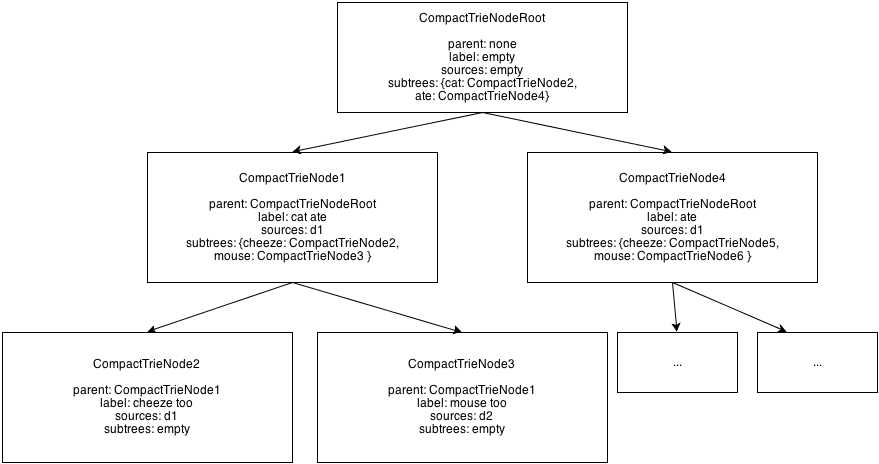
\includegraphics[totalheight=0.3\textheight]{Figures/compacttriedatastructure}
  \end{center}
  \caption{A simplified diagram of the compact trie data structure using two snippets “cat ate cheese” (d1) and “cat ate mouse too” (d2).}
  \label{fig:compacttriedatastructure}
\end{figure}

\subsubsection{Base clusters}
\label{subsubsec:baseclusters}
The \CTC algorithm generates base clusters with a simple recursive function. The function is called and applied to the root node of the compact trie. The function then creates new base clusters for each subtree in the root, and the subtrees of those subtrees etc. When all subtrees have been explored, the function recursively adds the sources of each subtree to their parent base cluster as the function climbs out of the recursion. This way each base cluster's sources (given a node in the compact trie) is the union of all the sources in the descendant nodes.

The algorithm then sorts the base clusters according to the base cluster scoring function. Many scoring functions are conceivable. The \emph{Order descending} parameter reflects the opposite scoring functions used for comparison in \cite{Moe2014}. In this thesis the scoring function is implemented as a sorting function to score clusters according to best or worst scores first. The order is given by the \emph{Order descending} parameter. \cite{Moe2014,Moe2013compact} show that the scoring of base clusters are sensitive to the kind of text that is being clustered. It is shown that ordering the base clusters in an ascending order (i.e. bottom or wort base clusters first) give better results for the ``Klimauken'' corpus. \cite{Oren1998} conversely use a descending order for base clusters were longer effective label lengths scores higher. The order of the base clusters should therefore be considered a worth while parameter for optimisation. Future research into the algorithm design of the \CTC algorithm could look into other possible scoring functions that use other base cluster characteristics. After selecting the top base clusters the algorithm design can take two forms: the first form specifying that singleton base clusters should be dropped, and the second form keeping singleton base clusters.

Recall the function for calculating the effective length of a base cluster label \(f(P)\) where \(f(P) = 0\) for \(length < 2\), \(f(P) = length\) for \(2 \le length < 7\), and \(f(P) = 7\) for \(7 < length \). Here the value 2 and 7 have been replaced by dynamic parameters \emph{min and max limits for base cluster scores}. The lower limit is a number in the range 0 \dots 20; the max limit a number in the range 3 \dots 25. If a corpus yields base clusters with generally longer labels, this will allow labels of longer lengths to be scored differently. A higher min limit will reduce the number of base clusters with short labels that might else wise be used in cluster creation.

The effective length of a label depends on the document frequency of each word in that label. A word contributes to a labels length if it satisfies two document frequency constraints. It should according to \cite{Oren1998} have a document frequency of at least 4, and occur in no more than 40\% of the collection's documents. Because word frequencies vary in different corpora the optimal parameters for each of the limits might also vary. For this reason each limit has been made a parameter for the optimisation algorithm. The \emph{min term occurrence} ranges from 5 to 150, and the \emph{max term ratio} from 0.05 to 1 with increments of 0.01.

\subsubsection{Base cluster merging}
\label{subsubsec:baseclustermerging}
Recall that \cite{Oren1998} merge base clusters using the ratio of common elements in the clusters, to the number of elements in the union of the two base cluster sets. This implementation is fairly naive because it only considers the amount of sources the base clusters share. The implementation produces big clusters with good source overlap (number of shared sources), but runs the risk of producing clusters with low label overlap (few shared label words). This original similarity measure only takes into account whether the two base clusters have some ratio of documents in common. In this thesis and in research by \citeauthor{Moe2014,Moe2014future} additional \emph{similarity measures} have been investigated. This thesis will concern itself with three alternative similarity measures.

The first alternative, Jaccard similarity, is based on the Jaccard similarity coefficient which was explained in Chapter~\ref{Theory}. It is quite similar to the Etzioni similarity measure, and as we will later see produce very similar results. Jaccard similarity will not be further discussed here. The second similarity measure, in this text called cosine similarity, incorporates the Vector Space Document model into the \CTC algorithm. Finally a third similarity measure based on the original Etzioni similarity measure was explored. In this measure the frequency of the base cluster labels were included in addition to the document overlap.

The similarity measure based on cosine similarity use the Vector Space Document model and cosine similarity function to find the similarity of base cluster labels. In this context a term's weight (tf-idf) is calculated not using it's document frequencies, but rather it's base cluster frequencies. Given a base cluster \(b\), the concatenation \(S^+\) of \(b\)'s documents, and the corpus collection \(C\) the tf-idf score of a given term \(t\) in \(b\)'s label can be calculated with the function \parencite{Moe2014}:

\begin{displaymath}
\vec{v}(t) = \left\{
  \begin{array}{l l}
    \text{tf-idf}(t, S^+, C) & \quad \text{if $t \in b$}\\
    0 & \quad \text{otherwise}
  \end{array} \right.
\end{displaymath}

Two base cluster labels are similar iff their cosine similarity is greater than some \(\theta_{cos}\). The cosine similarity of the two labels are calculated using the function below:

\begin{displaymath}
\frac{\sum_{t}\vec{v}(t) * \vec{v}'(t)}
{\sqrt{\sum_{t}\vec{v}(t)^2} * \sqrt{\sum_{t}\vec{v}'(t)^2}}
\ge \theta_{cos}
\end{displaymath}

A \(\theta_{cos}\) close to 1 will prevent base clusters from being merged, whilst a value close to 0 would allow close to all base clusters satisfying Etzioni similarity to be merged. Finding the right \(\theta_{cos}\) should therefore be part of the optimization task.

The third similarity measure, for convenience sake named Amendment similarity, also use the label of base clusters when determining the similarity of two base clusters. It is investigated in a future paper \citetitle{Moe2014future}, \parencite{Moe2014future}. Two base clusters are similar iff they are Etzioni similar, the average corpus frequency \(cf(w)\) of their label words are below some threshold \(\theta avg\), and that they share at minimum \(\theta min\) number of label words, \parencite{Moe2014}. The amendment can be expressed mathematically, where \(w\) represent a label word, as:

\begin{displaymath}
\frac{\sum\limits_{w \in b \cup b'} cf(w)}{\vert b \cup b' \vert} < \theta avg \quad \text{and} \quad \vert b \cap b' \vert > \theta min
\end{displaymath}

This similarity measure aims to capture those base cluster pairs whose labels indicate that the merged cluster would be extremely general. That is base cluster pairs whose average corpus frequency are higher than some threshold considered average for the collection. The measure also attempts to filter out those clusters that does not share label words.

Merging the base clusters produces a list of merged base clusters, or components. Each component is essentially a doubly linked list of base clusters. These components are converted to final clusters by collecting the sources and labels from the base clusters, and additionally measuring the source and label overlap of the cluster. The source overlap is the number of common sources in the base clusters in the component.

After merging base clusters into component clusters, the algorithm can drop or keep one word clusters. This is determined by the \emph{Drop one word clusters} parameter, and is included for reasons explained by \cite[][664]{Moe2014}: ``\textit{There will inevitably be clusters cemented by the co-occurrences of a single common word. Such clusters are often large and inaccurate. A one-word cluster is not necessarily a bad cluster but it seems reasonable to assume that this is the case more often than not.}''.

\subsubsection{Component Merge Implementation}
\label{subsubsec:componentmerge}
In the component merge step two components are merged by computing the union of the base cluster set in the first component and the base cluster set in the second component. There are a few ways to implement this with varying time complexities. While the original implementation, described below, worked well for previously investigated algorithm designs, tests revealed that some algorithm designs would produce components that would make the implementation extremely slow. It was therefore absolutely necessary to investigate alternative implementations for the merge step to make extensive algorithm design tests feasible.

The first implementation that was investigated uses a list implementation to store base clusters in the components. The implementation use a naive double for loop to find the union. For each base cluster in the second component the algorithm loops through the list of base clusters in the first component to check if the base cluster exists. If this is the case, the algorithm can store the common base cluster. The worst case time complexity of this algorithm is \(O(n*m)\) where \(n\) is the number of base clusters in the second component, and \(m\) the number in the first component. In some cases \(n\) and \(m\) can be almost equally big thus producing a quadratic time complexity. What this in practice means is that some parameter sets can have merge steps running for hours on end for very big base cluster amounts and low merge thresholds.

To solve this problem two additional implementations were investigated. The first attempt at a solution use simultaneous iteration over the two lists. This is done by first sorting the lists of base clusters (an at worst \(O(n \log n)\) operation). When the lists are sorted (by the base clusters' IDs) one can iterate through the lists simultaneously and make sure that there is no id from component 2 that is less than the the current id from component 1. This would mean that the base cluster from component 2 did not exist in component 1. This yields a time complexity of \(O(m)\) or \(O(n)\) depending on the length of the lists. This implementation thus works very well when \(n\) and \(m\) is relatively equal in size. For small values of \(n\) and large values of \(m\) it is still a good deal faster than the \(O(n*m)\) implementation, but not fast enough.

\begin{lstlisting}[float=ht, language=python, breaklines=true, label=lst:simultaneousmerge, caption={Simultaneous merge of components.}] 
base_clusters_2 = list(component2.base_clusters)
base_clusters_1 = list(component1.base_clusters)
list.sort(base_clusters_1, key=lambda bc_tuple: bc_tuple[0])
list.sort(base_clusters_2, key=lambda bc_tuple: bc_tuple[0])

i = 0  # base_clusters_1 counter
j = 0  # base_clusters_2 counter
base_clusters_add = []

while j < len(base_clusters_2):
  if i < len(base_clusters_1):
    id_1 = base_clusters_1[i][0]
    id_2 = base_clusters_2[j][0]

    if id_2 < id_1:  # This base cluster is not in base_clusters_1
      base_clusters_add.append(base_clusters_2[j])
      j += 1
    elif id_2 > id_1:  # There might be a base cluster in base_clusters_1
      i += 1
  else:  # They are the same, iterate both lists
    i += 1
    j += 1
else:  # No more base_clusters_1, add rest of two
  if id_2 != id_1:
    base_clusters_add.append(base_clusters_2[j])
    j += 1

for base_cluster in base_clusters_add:
  heappush(component1.base_clusters, base_cluster)
\end{lstlisting}
   
The second and final attempt at a solution use the dictionary class in Python to achieve lower time complexities. Each component implements its set of base cluster as a dictionary where the key is the base cluster's id (an integer) and the value is the base cluster object itself. The worst case time complexity of the dict object is linear time, \(O(n)\) for insert and get operations.\footnote{\href{https://wiki.python.org/moin/TimeComplexity}{TimeComplexity - Python Wiki}}. If the dict object consistently performed at worst case time complexity the run time of the algorithm would be the same as with the old list based implementation. Because the algorithm has no run time requirement for each base cluster insertion or base cluster check the worst case time complexity is not very important. Instead we can look at the average case time complexity to determine the suitability of the data structure. The average time complexity for both the insert and the get operations in the dict type are \(O(1)\). The time complexity of the get operation for dict objects is thus considerably much lower than that of the list type which is \(O(n)\). The time complexity of inserting the base clusters into the component would thus be an \(O(n)\) rather than an \(O(n \log n)\) operation. The merge operation would have a guaranteed time complexity of (on average) \(O(n)\). This ensures that the merge process runs fast even for large \(m\) and small \(n\) values.

\subsection{Genetic Algorithm}

As previously discussed the genetic algorithm is designed to follow the specifications in \cite{Goldberg1989,Negnevitsky2002,Haupt2004a}. The genetic algorithm itself is designed as a class and has a constructor which accepts configurable settings for things like population size, mutation rate, selection rate (keep size) and selection type. Additionally it requires a database handler with which it can store results. The genetic algorithm constructor generates an initial population of the specified size.

The evolution stage has been divided into a few operations. First the algorithm calculates generational data. This includes the average fitness of the chromosomes, average numbers for the different performance measures namely: precision, recall, and F-Measure. The average scores and scores held within the top, bottom and median chromosomes are all stored in a MySQL database.

After that comes the ``generation step'' which performs the evolution itself. It starts by discarding the bottom chromosomes given by the keep size. The remaining chromosomes are then used for mating. The algorithm only implements the roulette wheel selection type. Offspring are produced by slicing the parameter set in the two parent chromosomes and then combining the first and last halves respectively to form two new chromosomes.

After creating the offspring a random selection of the chromosomes in the entire population are mutated. The mutation rate and number of genes determine the number of mutations that occur in the population. The last step takes the offspring chromosomes and those chromosomes that were mutated and sends them to the task organiser which is responsible for creating clustering tasks and sending them to the clustering algorithm clients.

The \texttt{Chromosome} class models a chromosome in the genetic algorithm. It contains a number of genes (see Listing~\ref{lst:chromosome}) which also act as the algorithm design and respective parameters for the \CTC algorithm. The constructor of the \texttt{Chromosome} class takes each parameter as a constructor parameter. The \texttt{calc\_fitness\_score} method applies itself as an argument to a cluster method in a \texttt{CompactTrieClusterer} object. In this way it sends the \CTC parameters to the clustering algorithm. The \texttt{cluster} method in the \texttt{CompactTrieClusterer} object in turn insert the clustering result into the chromosomes result property. The \texttt{calc\_fitness\_score} function then use the cluster results F-Measure score and a modifier to calculate its own fitness. See Listing~\ref{lst:chromosomefitness} for details. The modifier works as a balancer that prevents the genetic optimisation algorithm from producing algorithm designs that generates too many clusters.

\begin{lstlisting}[float=ht, language=python, breaklines=true, label=lst:chromosomefitness, caption={Fitness function in the Chromosome class.}]
def calc_fitness_score(self, compact_trie_clusterer):
    """
    Returns the fitness of the chromosome

    Args:
        cSetting (clusterSettings): An object wrapping data
        and settings needed to run the clustering algorithm,
        the parameters in chromosome excluded.
    """
    self.result = compact_trie_clusterer.cluster(self)
    precision0 = self.result.precisions[0]
    recall0 = self.result.recalls[0]

    ratio_modifier = 0

    if self.result.no_of_gt_clusters > 0:
        cluster_ratio = (self.result.no_of_clusters / self.result.no_of_gt_clusters)
        if 0.8 <= cluster_ratio <= 3:
            ratio_modifier = 0.1
        else:
            ratio_modifier = -0.1

    self.fitness = self.result.f_measures[0] + ratio_modifier
\end{lstlisting}

The chromosome module additionally implement a cross over function for producing offspring. This can be seen in Listing~\ref{lst:crosschromosomes}. It takes two chromosomes and retrieves their genes as tuple objects. It then crosses them by calculating a random cross over point and slicing the tuples at that position. The function then calls the \texttt{genes\_tuple\_to\_chromosome} function to create two new chromosomes for the new genes.

\begin{lstlisting}[float=ht, language=python, breaklines=true, label=lst:crosschromosomes, caption={Code for crossing chromosomes}]
def crossChromosomes(chromosome1, chromosome2):
    """
    Takes two  parent chromosomes cross them and return two children
    chromosomes
    """
    genes1 = chromosome1.genesAsTuple()
    genes2 = chromosome2.genesAsTuple()
    crossOverPoint = randint(1, len(genes1) - 1)
    genes12 = genes1[0:crossOverPoint] + genes2[crossOverPoint:len(genes2)]
    genes21 = genes2[0:crossOverPoint] + genes1[crossOverPoint:len(genes1)]

    return [genesTupleToChromosome(genes12),
            genesTupleToChromosome(genes21)]
\end{lstlisting}

\subsection{Distribution framework}
The \CTC algorithm performs rather slowly because of its \(O(n^2)\) base cluster merging step. The problem grows quadratically for the number \(n\) of base clusters. Adding to the problem of optimisation is the fact that genetic algorithms can use a long time to find optimised solutions if the population size is too big. To make larger optimization tasks feasible a distribution framework was implemented. The distribution framework also has the added benefit of making it easy to utilise all CPU cores by running one client for each one. Chapter~\ref{EvaluationTesting} will show how it is feasible to run the optimization on a single computer.

The framework consists of two parts: a server, and a client. The server handles all communication between itself, the clients and the genetic algorithm. It consists of the following main classes: \texttt{Server}, \texttt{ClientHandler}, \texttt{TaskOrganizer}, and a \texttt{ScoreBoard}. The server instance handles incoming connections and creates ClientHandler instances to communicate with the clients. Very basic authentication of clients are performed before the client is permitted to join the computation tasks. A client instance will send a task request message to the client handler. Upon acquisition of the message the client handler will ask the task organiser for available clustering tasks. If any tasks are available it will send these to the client handler. The client will then use a \texttt{CompactTrieClusterer} object to perform the clustering task and send the results back to the client handler.

The task organiser keeps a timeout index of all tasks given to a client handler. If a task has been in this index for a certain amount of time, the task will be put back into the list of available tasks. This ensures that tasks that never would have finished can be given to other clients. The score board tracks the number of completed tasks per user. It was implemented to facilitate a competetive environment with regards to computation of tasks among users contributing computing power.

Once all the tasks have been completed the task organiser notifies the genetic algorithm. The genetic algorithm then initiates its evolution method. When the genetic algorithm has finished creating a new generation of offspring, it creates new clustering tasks which is added to the list of available tasks. This cycle continues until the genetic algorithm meets a cutoff criteria. In our implementation of the genetic algorithm the genetic algorithm stops the generation loop if the best performing chromosome does not change for 10 generations. If the same chromosome achieves the best fitness for ten consecutive generations one can be pretty sure that the algorithm has converged on that optimum. See the source code for a detailed look at how the interaction between the software components occurs.